% This is the Reed College LaTeX thesis template. Most of the work
% template. Later comments etc. by Ben Salzberg (BTS). Additional
% restructuring and APA support by Jess Youngberg (JY).
% Your comments and suggestions are more than welcome; please email
% them to cus@reed.edu
%
% See http://web.reed.edu/cis/help/latex.html for help. There are a
% great bunch of help pages there, with notes on
% getting started, bibtex, etc. Go there and read it if you're not
% already familiar with LaTeX.
%
% Any line that starts with a percent symbol is a comment.
% They won't show up in the document, and are useful for notes
% to yourself and explaining commands.
% Commenting also removes a line from the document;
% very handy for troubleshooting problems. -BTS

% As far as I know, this follows the requirements laid out in
% the 2002-2003 Senior Handbook. Ask a librarian to check the
% document before binding. -SN

%%
%% Preamble
%%
% \documentclass{<something>} must begin each LaTeX document
\documentclass[12pt,twoside]{reedthesis}
% Packages are extensions to the basic LaTeX functions. Whatever you
% want to typeset, there is probably a package out there for it.
% Chemistry (chemtex), screenplays, you name it.
% Check out CTAN to see: http://www.ctan.org/
%%
\usepackage{graphicx,latexsym}
\usepackage{amsmath}
\usepackage{amssymb,amsthm}
\usepackage{longtable,booktabs,setspace}
\usepackage{chemarr} %% Useful for one reaction arrow, useless if you're not a chem major
\usepackage{rotating}

% Modified by CII
\usepackage[hyphens]{url}
\usepackage{hyperref}
\usepackage{lmodern}

% Added by CII (Thanks, Hadley!)
% Use ref for internal links
\renewcommand{\hyperref}[2][???]{\autoref{#1}}
\def\chapterautorefname{Chapter}
\def\sectionautorefname{Section}
\def\subsectionautorefname{Subsection}

\usepackage{caption}
\captionsetup{width=5in}

% \usepackage{times} % other fonts are available like times, bookman, charter, palatino

\title{}
\author{}
% The month and year that you submit your FINAL draft TO THE LIBRARY (May or December)
\date{}
\division{}
\advisor{}
%If you have two advisors for some reason, you can use the following
%%% Remember to use the correct department!
\department{}
% if you're writing a thesis in an interdisciplinary major,
% uncomment the line below and change the text as appropriate.
% check the Senior Handbook if unsure.
%\thedivisionof{The Established Interdisciplinary Committee for}
% if you want the approval page to say "Approved for the Committee",
% uncomment the next line
%\approvedforthe{Committee}

% Below added by CII

%%% Copied from knitr
%% maxwidth is the original width if it's less than linewidth
%% otherwise use linewidth (to make sure the graphics do not exceed the margin)
\makeatletter
\def\maxwidth{ %
  \ifdim\Gin@nat@width>\linewidth
    \linewidth
  \else
    \Gin@nat@width
  \fi
}
\makeatother

\renewcommand{\contentsname}{Table of Contents}

\setlength{\parskip}{0pt}


\providecommand{\tightlist}{%
  \setlength{\itemsep}{0pt}\setlength{\parskip}{0pt}}

\Acknowledgements{

}

\Dedication{

}

\Preface{

}

\Abstract{

}


%%
%% End Preamble
%%
%

\begin{document}

  
  \frontmatter % this stuff will be roman-numbered
  \pagestyle{empty} % this removes page numbers from the frontmatter

  
  
  % Add table of abbreviations?

      \hypersetup{linkcolor=black}
    \setcounter{tocdepth}{1}
    \tableofcontents
  
  
  
  
  
  \mainmatter % here the regular arabic numbering starts
  \pagestyle{fancyplain} % turns page numbering back on

  \chapter*{Introduction}\label{introduction}
  \addcontentsline{toc}{chapter}{Introduction}
  
  Knock Software's \emph{Ride Report} app combines a simple
  thumbs-up/thumbs-down rating system with GPS traces of bicycle rides to
  compile a crowdsourced data set of which routes are and are not
  stressful for urban bicyclists.
  
  The app that collects the data is simple: \emph{Ride Report}
  automatically detects when a user start riding their bike, records the
  GPS trace of the route, and then prompts the user at the end of the ride
  to give either a thumbs-up or thumbs-down rating. From this, they were
  able to create a simple ``stress map'' of Portland, OR, which displays
  the average ride rating of rides going through each discretized ride
  segment.
  
  \begin{figure}[h!tbp]
  \centering
  \includegraphics[angle = 0,scale = 0.75]{figure/stress_map.jpg}
  \caption[Ride Report's Stress Map for Portland. Greener road segments incidate less
  while more red segments indicate more stressful streets. ``Stress'' computed by
  taking the average rating for each segment.]{\normalsize{Ride Report's Stress Map for Portland. Greener road segments incidate less
  while more red segments indicate more stressful streets. ``Stress'' computed by
  taking the average rating for each segment.}}
  \label{fig:stress-map}
  \end{figure}
  
  The app privileges reducing barriers to response to increase sample size
  over ensuring quality and consistent responses. This presents the first
  problem: how can we analyze ratings when riders are likely rating rides
  inconsistently?
  
  At the same time, we have another challenge. We have ratings associated
  with routes, but we would like to know the effect of particular road
  segments, for both inference (what effect does this road segment have on
  the rating?) and prediction (given a route, what do we expect the rating
  to be?) purposes.
  
  Finally, there are interesting issues with missing data. First, the
  sample of rides we have are biased towards routes that riders percieve
  as better. Second, a significant portion of the rides are missing a
  response, and non response is unlikely to be independent of the
  response. The good news is that we have all the predictors for every
  ride, enabling us to build a model that is able to leverage the data
  with missing responses rather than listing the missing data as a
  liability.
  
  \section{Accounting for Rider Rating
  Variance}\label{accounting-for-rider-rating-variance}
  
  For ratings we are interested in modeling variance between riders (as we
  might expect riders to have different rating patterns than their peers)
  and within riders (as riders may not rate the same route and conditions
  the same every time). To model this, we propose using multilevel
  regression, with random effects from each rider. This approach has been
  used in similar situations, in one case to model sexual
  attraction\footnote{Mackaronis et al. (2013)}.
  
  In a multilevel model, we fit a regression where the intercept term
  varies by group but comes from a common distribution. For example, if we
  let \(r_i\) be the rating of the \(i\)th ride, \(X_i\) be the ride-level
  variables, then we can fit a regression:
  
  \[\mathbb{P}(r_i = 1) = \text{logit}^{-1}
  \left( \alpha_{j[i]} +  X_i \beta \right) ,\] where \(\alpha_j\) is an
  intercept specific to rider \(j\). In addition, the rider intercepts
  come from a common distribution,
  \[\alpha_j \sim N (\mu_\alpha, \sigma^2_\alpha),\]
  
  where \(\mu_\alpha\) is the mean of all the \(\alpha_j\)s.
  
  Using varying intercepts will allow our model to exhibit the property of
  varying rates of riders giving stressful ratings. This can be extended
  to model differences in how riders respond to different kinds of road
  conditions using varying slope models. We explore multilevel model
  further in Section \autoref{h-models} and multilevel models for riders
  in Section \autoref{add-riders}.
  
  \section{Addressing Road Segments as a
  Level}\label{addressing-road-segments-as-a-level}
  
  We examine multiple approaches to modeling road segments. In the first,
  we regard add regression term for the route, that is a weighted sum of
  terms for each road segment in the route, weighted by the lengths of the
  segments. The terms for the
  
  the contribution of the route to be a weighted sum of the contributions
  of road segments in the route, weighted by the lengths of the segments.
  
  \section{Approaching Missing Data at Multiple
  Levels}\label{approaching-missing-data-at-multiple-levels}
  
  This data set contains missing data at two levels.
  
  First, there are many routes without any ratings. The routes taken by
  riders are not a random sample of routes, but are often already chosen
  by the rider as the least stressful ride. As we might expect because of
  this bias, only a small proportion of rides are rated as ``stressful.''
  
  One solution we explore to this problem is adding a segment popularity
  parameter as a segment-level predictor.
  
  Second, not every ride is given a rating. We do have the route they
  chose, and all associated covariates, but the response variable, rating
  is missing. As we will discuss in chapter \autoref{missing-data}, the
  pattern of non-response is unlikely to be unbiased.
  
  To address the second problem, we first build a separate probability
  model that predicts non response, and then integrate that model into our
  main model.
  
  \chapter{Data Sources}\label{data-sources}
  
  We combine several data sources to do our analysis. Information about
  individual rides, including the GPS trace, the rider, and start
  timestamp were provided by Ride Report. Weather data were collected from
  Weather Underground's archive of the KPDX weather station and a Portland
  Fire Bureau station.
  
  Our goal in this chapter is to discuss this data and what considerations
  we should have in mind before exploring it in depth. This includes how
  and by whom the data was collected, who and what is this data actually
  representative of, and what samples were taken of the data.
  
  Some of these considerations, such as the limited demographics
  represented in the Ride Report data, pose serious limitations to how our
  inferences can be generalized. Others, such the large number of missing
  responses in the Ride Report data, motivate the analysis we are doing in
  this thesis. Finally, there are other considerations which we will
  acknowledge here, but addressing them is out of the scope of this
  thesis. This data set contains an abunance of potential research
  questions, only a fraction of which could be reasonably addressed in one
  thesis.
  
  \section{Ride Report}\label{ride-report}
  
  Ride Report's data is the focus of this paper. Knock Software created
  the app to collect large amounts of information about urban cyclists'
  routes and experiences on those routes. The hope is that this
  information will be valuable to city planners.\footnote{Knock's other
    project is making a cheaper bicycle counter for cities to monitor
    traffic flow, again intended to be sold to cities wishing to improve
    bike infrastructure.}
  
  Ride Report's approach to crowdsourcing this data is particularcly
  important to understand. The app automates every piece of the data
  collection process except for the rating given by the rider. Thus, the
  app casts aside nuanced and (somewhat) reliable human input in favor of
  increasing sample size (i.e.~one could imagine a similar app where users
  have more control over how the route is recorded, have the ability to
  rate on a more fine-grained scale, and are given more direction in what
  they are rating for.) This leads to some potential issues that we need
  to address in our models.
  
  Before we get into the potential issues in the data collection, let's
  examine the data collection process itself. When installed on a persons
  phone, the Ride Report app attempts to automatically detect when the
  user starts riding their bicycle, based acceleromoter data, when a user
  leaves a familiar Wi-Fi network, and some other pieces of information.
  When the app detects the start of a ride, it starts recording a GPS
  trace. At the end of the users ride, the app detects them getting of
  their bike (in a similar process to how it detected the start of a ride)
  and prompts them to give a rating of the ride. The ride data is saved
  then, even if the user does not provide a rating.
  
  This automatic detection of when a ride starts and stops leads to two
  related and common errors in the dataset: first, one ride is often split
  into two or more rides at points, such as at a stoplight or a train
  crossing, where a cyclist stops for an extended period of time; second,
  car rides are sometimes misclassified as bicycle rides and vice-versa
  (car rides are not rated.) The app does allow riders to correct the
  misclassification, but there is currently no way to join split rides
  back together (Knock is working on changing that, though.)
  
  \begin{figure}[tbh]
  \centering
  \includegraphics[angle = 0,scale = 0.35]{figure/ride_report_rating.jpg}
  \caption[The Ride Report app's interface has changed significantly between
  versions, including the rating text displayed after a ride. This is the current
  version as of Februrary 2015.]{\normalsize{The Ride Report app's interface has changed significantly between
  versions, including the rating text displayed after a ride. This is the current
  version as of Februrary 2015.}}
  \label{fig:ride-rating}
  \end{figure}
  
  The app only recently became publicly availible and has undergone
  significant changes in the course of it's life. In particular, while the
  ratings have always been binary, the labels have changed at various
  points in time. For a while the rating labels were ``Stressful'' and
  ``Chill'', while now they are labelled ``Recommend'' and ``Avoid'' (see
  \autoref{fig:ride-rating}.) Other fundamentals of the data collection
  process, have remained constant, however.
  
  The data colletion method itself has some problems, but there also may
  be some biases in the population of riders using the app. The app is
  only availible on iOS, so only iPhone owners could use this application
  which may imply a bias toward riders of higher socioeconomic status. At
  the time of the start of the thesis, the app was in private beta,
  meaning only people who actively sought out using the app were able to
  use it. Now the application is public and on the Apple App Store, making
  it more widely availible. So many of the earlier rides may be people
  within the developer's personal network. Unfortunately, it's hard to
  make any solid conclusions about the users of the app because Ride
  Report doesn't collect any demographic data about their riders.
  
  One other issue with the Ride Report data guided our analysis: privacy.
  Because the data involves timestamps and GPS locations of people's
  commutes, the data is very sensitive: one could easily infer someone's
  home and workplace based on their most commons routes. In fact, this
  data is protected by an end-user license agreement (EULA) which prevents
  sharing of data, without the explicit permission of those involved. This
  presented a logistic challenge: how were we to do inference and data
  exploration without access to the data?
  
  By agreement with Knock Software, identifying data must be kept private.
  With permission from five riders, Knock was able to give us a small
  subset consisting of all the rides from those five riders, to be kept
  confidential. That is the data set we used for prototyping models and
  some basic exploratory analysis. Knock also agreed to allow us to run
  models fitting scripts on larger samples of their dataset, as long as
  they were performed on their computers, with no identifying data leaving
  their system.
  
  While at first this set up seems like an inconvenience, it actually has
  some advantages. One of the pitfalls of having an entire data set,
  especially a high dimensional one, is that in performing exploratory
  analyses it is often too easy to find spurious ``statistically
  significant'' results. Instead, we must come up with our models before
  running them, greatly limiting the choices we can make in the garden of
  forking paths.
  
  \section{Weather Data}\label{weather-data}
  
  Slippery roads and formidable winds are no fun for anyone balancing on a
  two-wheeled vehicle. Weather is, then, one of the most obvious family of
  predictors for ride rating, at least intuitively. We use the time of a
  ride to join in data about the weather conditions during the ride,
  including
  
  \begin{itemize}
  \tightlist
  \item
    the temperature,
  \item
    whether and how much it is raining,
  \item
    whether the roads are wet or have puddles,
  \item
    wind and gust speed.
  \end{itemize}
  
  We include the first two, temperature and percipitation, to account for
  rider comfort. A swealtering, frigid, or stormy day could make an
  unpleasant experience for a bicyclist and thus could lead to more
  negative ratings.
  
  On the other hand, we include the last two, wet road and gust speed, as
  factors that impact safety. During and after storms, puddles often
  accumulate in bike lanes before the center of the road, pushing cyclists
  into lanes shared by cars, which are often more dangerous.
  
  Gust speeds impact the aerodynamics of a ride, which are particular
  important for bicyclists. It's one of the main reasons cyclists care
  about getting into lower (and more aerodynamic) rider positions. Thus,
  high wind or gust speeds may affect rider rating.
  
  \begin{figure}[tbh]
  \centering
  \includegraphics[angle = 0,scale = 1]{figure/weather_station_map.pdf}
  \caption[Positions of weather data collection sites. Daily weather information
  was collected at the KPDX weather station at Portland International Airport. 
  Hourly percipitation data was collected at the Portland Fire Bureau's rain
  guage in downtown Portland.]{\normalsize{Positions of weather data collection sites. Daily weather information
  was collected at the KPDX weather station at Portland International Airport. 
  Hourly percipitation data was collected at the Portland Fire Bureau's rain
  guage in downtown Portland.}}
  \label{fig:weather-stations}
  \end{figure}
  
  We are limiting our study to rides in Portland, Oregon. Given this, we
  can first assume that it may be reasonable to expect that riders are
  used to the same climate, and thus have somewhat similar responses to
  weather. This also makes it reasonable to use data from one nearby
  weather station, rather than attempting to collect from several stations
  and creating a spatial model for weather.
  
  For daily summaries of weather conditions, we used weather history from
  the KPDX weather station at Portland International Airport downloaded
  from Weather Underground. From this we were able to get daily weather
  data, including
  
  \begin{itemize}
  \tightlist
  \item
    Average, minimum, maximum temperature for the day.
  \item
    Total percipitation.
  \item
    Mean wind speed, as well as gust speed (speed of brief, strong winds.)
  \end{itemize}
  
  We also got hourly rainfall data from a data stream at the Portland Fire
  Bureau Rain Gage at 55 SW Ash St., which is just about the geographic
  center of Portland. This just gives raw uncorrected rain guage data, but
  gives us a fine grain look at how much rain there has been recently.
  
  For daily weather data, such as temperature highs and average wind
  speed, we use information from the KPDX weather station. This weather
  station is the best calibrated in the area. It is further from the
  geographic center of the rides we are examining, but because the weather
  is daily summary statistics, we don't expect closer weather stations to
  be much more informative. \autoref{fig:weather-stations} shows the
  geographic positions of these two stations.
  
  \section{Our Predictors}\label{our-predictors}
  
  We combined the ride records with weather data by joining by start
  datestamp of the ride. We will denote our set of ride-level predictors,
  each of which is a column vector as, - \(x^\text{length}\), ride length,
  scaled to have mean 0 and standard deviation of 1 - \(x^\text{rain}\),
  rainfall during hour of ride, in tenths of inches - \(x^\text{rain4h}\),
  rainfall during past four hours before ride, in tenths of inches -
  \(x^\text{wind}\), mean wind speed for the day, in miles per hour -
  \(x^\text{gust}\), max gust speed for the day, in miles per
  hour\footnote{Gust speeds are the max speeds of winds that are fast,
    highly variable, and short-term. For METAR weather stations, which the
    KPDX station is, gust speeds report the maximum wind speed when there
    were rapid fluxations in wind speed with at least 10 knots in the
    difference between the lows and highs.} - \(x^\text{temp}\), average
  temperature, in degrees Fahrenheit for the day.
  
  We will often represent this set of predictors as the ride-level
  predictor matrix
  \(X = (x^\text{length} \; x^\text{rain} \; x^\text{rain4h} \; x^\text{wind} \; x^\text{gust}\; x^\text{temp}).\)
  We also have the predictor \(t \in [0, 24]^n\), representing the time of
  day of the ride, measured by hours since midnight. (Because of it's
  special role in building our models, we use the simple notation of a
  single letter for it.)
  
  Let \(Y_i = 1\) if the \(i\)th ride received a negative rating, and
  \(Y_i = 0\) if it received a positive rating. Choice of coding which
  events are 0's and which are 1's is arbitrary when making logistic
  regression models, though we made this choice because for the sake of
  our analysis, negatively rated rides are more interesting events. For
  urban planning applications, they define the areas that need attention.
  
  \chapter{Methods}\label{methods}
  
  In building our models, we use a multitude of statistical methodologies.
  We outline here the central methods used, both to familiarize the reader
  and to establish the notation we use throughout this paper.
  
  Statistics is often split up into prediction and inference. Both are
  important to us here: we use inference to answer our research questions
  and prediction---through cross validation---to evaluate the validity of
  our models.
  
  Our models combine logistic regression and multilevel regression. To
  evaluate our models, we use graphical tools, such as the separation
  plot, to examine the performance.
  
  \section{Logistic Regression}\label{logistic-regression}
  
  Statistical models are often split into regression models---models with
  a quantitative response---and classification models---models with a
  categorical response. Thus, it may seem odd that we are using a
  regression model when our response variable, ride rating, is a binary
  outcome.
  
  But, when modeling a binary variable \(Y\), we consider it a Bernoulli
  random variable, \[Y = \text{Bernoulli}(p),\] where \(p\) is the
  probability the outcome is 1 and \(1-p\) is the probability the outcome
  is 0. So our outcome variable \(Y\) may be binary, but the primary
  quantity of interest behind that outcome is \(p\), a quantitative
  variable. This is why we consider logistic regression a regression
  method.
  
  Logistic regression is one form of generalized linear regression. Recall
  that in linear regression we use data with response variable \(y_i\) and
  \(j\) predictors \(x_{i1}, \ldots, x_{ij}\) to fit the best-fitting
  linear function
  
  \[y_i = \beta_0 + \beta_1 x_{i1} + \cdots + \beta_j x_{ij} + \epsilon,\]
  
  where \(\epsilon \sim N(0, \sigma^2)\), by estimating
  \(\beta_0, \ldots, \beta_j\). We can equivalently write,
  
  \[Y \sim N(\beta_0 + \beta_1 x_1 + \ldots + \beta_j x_j, \sigma^2).\]
  
  We could, in fact, try to predict \(p\) with a linear regression, though
  such a model will always have the problem of predicting probabilities
  outside of the range of \([0, 1]\). That's not a recipe for simple
  interpretation or reliable predictions. Generalized linear regression
  uses a ``link function,'' \(g\), to modify the regression so the range
  of the response more accurately reflects the practical range of the
  variable:
  
  \[g(y_i) = \beta_0 + \beta_1 x_1 + \ldots + \beta_j x_j + \epsilon.\]
  
  In logistic regression, the ``link'' function is the logit function,
  \(\text{logit}:[0,1] \to \mathbb{R}\),
  
  \[\text{logit} (p) = \log \left(\frac{p}{1-p}\right). \]
  
  This function is also known as the log-odds, because odds are defined as
  \(p/1-p\) for any probability \(p\).
  
  So in logistic regression, we model the probability of \(y_i = 1\) as,
  
  \[\mathbb{P} (y_i = 1) = \text{logit}^{-1} (\beta_0 + \beta_1 x_1 + \ldots + \beta_j x_j).\]
  
  Notice that the inverse logit function\footnote{sometimes called the
    logistic function} maps values from \(\mathbb{R}\) to \([0,1]\). Thus,
  the function provides a convenient way to map linear combinations of
  other variables onto values that are valid probabilities. Other such
  functions exist and are also used for regressions with binary responses,
  such as the probit function. Logistic regression, however, is easier to
  interpret and more efficient to compute.
  
  \begin{figure}[tbh]
  \centering
  \includegraphics[angle = 0,scale = 1]{figure/logit_plot.pdf}
  \caption[The inverse logit function gives a convenient way to map linear
  combinations of real numbers to valid probability values.]{\normalsize{The inverse logit function gives a convenient way to map linear
  combinations of real numbers to valid probability values.}}
  \label{fig:logit-plot}
  \end{figure}
  
  Though coefficients from a logistic regression can't be interpreted the
  same way as a linear model, they do have a convenient interpretation.
  Because the linear part of the model represents log odds, the
  coefficients are log odds ratios; That is, the exponentiated
  coefficients \(e^{\beta_1}, \ldots, e^{\beta_j}\) represent the
  multiplicative effect a one-unit increase in the corresponding predictor
  has on the odds. For example, if we fit a simple logistic regression
  with \(\mathbb{P}(Y = 1) = \text{logit}^{-1} (\alpha + \beta + X)\), we
  could interpret \(e^{\beta} = 1.1\) as meaning that a one unit increase
  in \(X\) gives a 10\% increase in the odds that \(Y = 1\).
  
  We started out talking about the ways logistic regression is both a
  classification and regression model. We will mostly care about logistic
  regression as a regression model. One of the main ways we will assess
  our models is through the accuracy of predictions. But, in the
  classification framework, in order to predict the outcomes \(\hat{Y}\),
  we need to choose a probability threshold to decide which outcome we
  should predict for a given observation. When we care mainly about
  prediction, this approach can make sense. Our interest, however, lies in
  prediction. So rather than choose an arbitrary threshold, we will
  evaluate the accuracy of our predicted probabilities themselves. (How
  exactly do we do this? See \autoref{evaluate}.)
  
  \section{Hierarchical Models and Mixed Effects Models}\label{h-models}
  
  Data often contain hierarchies. For example, a set of student test
  scores may contain the hierarchy of districts and schools those students
  attend. Or a set of soil samples may have been taken at several distinct
  sites, thus having a hierarchy of sites and samples. In the bike ride
  data we examine, there is the hierarchy of riders and rides.
  
  We will talk about different ``levels'' of variables corresponding to
  places in this hierarchy. When we refer to ``ride-level variables,'' we
  refer to variables that are specific to a ride, whereas we refer to
  ``rider-level variables'' as those specific to the rider, and thus also
  all the rides that rider takes. For example, we consider length a
  ride-level variable and total number of rides taken a rider-level
  variable.
  
  We will also discuss road segment-level variables, which are variables
  that are specific to the road segments in the route of a ride
  (e.g.~length, presence of bike lanes, etc). But there isn't a clear road
  segment-ride hierarchy: each ride contains multiple road segments and
  each road segment is contained by multiple rides. Thus, this isn't a
  case where multilevel modeling is applicable. (The ideas behind it,
  though, may be fruitfully adapted.)
  
  Gelman describes two traditional ways of dealing with hierarchical data
  that multilevel models contrasts with: ``complete pooling'' and ``no
  pooling.''\footnote{Gelman and Hill (2006), p.~7} In ``complete
  pooling,'' we ignore the group-level variables, and give identical
  estimates for parameters for every group. In ``no pooling,'' we do
  entirely separate regressions for each group. Multilevel models are a
  comprimise between these extremes (``partial pooling'', as Gelman calls
  it) where all the data is considered in a single regression with some
  parameters shared between groups and some different between groups.
  (This will become clearer when we introduce examples of models.)
  
  These multilevel models work for other forms of regression, but we will
  focus on logistic regression, as it is the method we use in this paper.
  We will be using notation adapted from Gelman and Hill's description of
  multilevel models.\footnote{Gelman and Hill (2006), p.~251--252}
  Consider a data set composed of
  
  \begin{itemize}
  \tightlist
  \item
    \(i\) observations of a binary response variable \(y_i\),
  \item
    \(m\) observation level predictors \(X_i = x_i^1, \ldots, x_i^m\),
  \item
    \(j\) groups in which the observations are split into,
  \item
    \(l\) group-level predictors
    \(U_{j[i]} = u_{j[i]}^1, \ldots, u_{j[i]}^l\), where \(j[i]\) is the
    group of the \(i\)th observation.
  \end{itemize}
  
  We could fit a model where the intercept varies by group:
  
  \[\mathbb{P} (y_i = 1) = \text{logit}^{-1}
  (\alpha_{j[i]} + X_i \beta),\]
  \[\alpha_{j[i]} \sim N(\gamma_0 + U_{j[i]} \gamma, \sigma_{\alpha}^2),\]
  
  where \(\alpha_{j[i]}\) is the intercept for the \(j\)th group,
  \(\beta\) is a vector coefficients for the observation-level predictors,
  \(\gamma_0\) are the group-level intercepts, and \(\gamma\) is a vector
  of coefficients for the group-level predictors. We could also specify a
  similar model where there are no group-level predictors, such that we
  simply have different intercepts for each group,
  \[\alpha_{j[i]} \sim N(\gamma_0, \sigma_{\alpha}^2),\]
  
  We can also consider a model that has slopes varying by group. For
  simplicity, let's consider just one observation-level predictor,
  \(x_i\), that will have varying slopes \(\beta_{j[i]}\) as well as one
  group-level predictor. We could specify the model as,
  
  \[\mathbb{P} (y_i = 1) = \text{logit}^{-1}
  (\alpha_{j[i]} + \beta_{j[i]} x_i),\]
  
  \[
  \left(
  \begin{array}{c}
  \alpha_{j}\\
  \beta_{j}
  \end{array}
  \right) =
  N \left(
  \left(
  \begin{array}{c}
  \gamma_0^\alpha + \gamma_1^\alpha u_j\\
  \gamma_0^\beta + \gamma_1^\beta u_j
  \end{array}
  \right),
  \left(
  \begin{array}{cc}
  \sigma^2_\alpha & \rho \sigma_\alpha \sigma_\beta\\
  \rho \sigma_\alpha \sigma_\beta & \sigma^2_\beta
  \end{array}
  \right)
  \right).
  \]
  
  \section{Tools for evaluating models}\label{evaluate}
  
  After fitting our models, we will want to know, how do each of our
  models compare? Did adding a particular term enhance or diminish the
  accuracy of our model? While we are fitting our models for inference, we
  will be evaluating them by the accuracy of their predictions. That is,
  how accurately and confidently can the model dicern which rides were
  rated as good and which as bad?
  
  The predictions we will evaluate will be done in the context of cross
  validation. Usually, we will just use a simpy 2-fold cross validation,
  where we split the data into two random samples, fitting the model on
  one set (the ``training set''), and using the model to predict on the
  other set (the ``testing set'') to check accuracy. We can also do
  \(k\)-fold cross validation, where we split the data into \(k\) samples,
  and for each of the samples we train the model with the other \(k-1\)
  samples and then test with the left out sample.
  
  When splitting the data into testing and training sets, we can not do a
  simple random sample. If we do, we will end up with riders in the
  testing set that aren't in the training set, which our models that use
  rider information cannot predict on. Thus, we will usually do stratified
  sampling of rides with riders as strata.
  
  When evaluating the predictions from a model, statistics such as
  classifications rate, false-positive rate, and true-negative rate can be
  calculated for each validation. For a more comprehensive look at
  predictive accuracy, we use the separation plot as well as homemade plot
  to assess our models.
  
  \subsection{The Separation Plot}\label{the-separation-plot}
  
  The separation plot, created by Greenhill et. al.\footnote{Greenhill,
    Ward, and Sacks (2011)}, is designed to show how well a logistic
  regression model can distinguish between high and low probability
  events.
  
  Creating a separation plot first requires a model fit to training data
  and testing data to evaluate predictive accuracy on. From the testing
  data, we need a vector \(Y\) of observed binary response data and a
  vector \(\hat{Y}\) of predicted probabilities of a 1 for each
  observation, predicted using our model fitted to training data.
  
  We plot the data \((Y, \hat{Y})\) as a sequence of vertical strips,
  colored according to observed outcome, \(Y\), and ordered from low to
  high probability based on \(\hat{Y}\). A curve is superimposed upon the
  stripes showing the \(\hat{Y}\) as a line graph. And finally, a small
  triangle is placed indicated the point at which the two colors of lines
  would meet if all observations \(Y = 0\) were placed to the left of all
  the \(Y=1\) observations; in other words, showing where the boundary
  would be if the two classes were perfectly separated by the model.
  
  \begin{figure}[tbh]
  \centering
  \includegraphics[angle = 0,scale = 1]{figure/sep_plot_examples.pdf}
  \caption[Above we have examples of three separation plots. The first plot shows
  what it looks like when $Y$ and $\hat{Y}$ are uncorrelated. The second plot 
  shows a fairly good model, where the $Y$ are generated as Bernoulli($\hat{Y}$).
  The third plot shows a model where the responses are fully separated.]{\normalsize{Above we have examples of three separation plots. The first plot shows
  what it looks like when $Y$ and $\hat{Y}$ are uncorrelated. The second plot 
  shows a fairly good model, where the $Y$ are generated as Bernoulli($\hat{Y}$).
  The third plot shows a model where the responses are fully separated.}}
  \label{fig:sep-plot-examples}
  \end{figure}
  
  Separation plots don't do well with larger sample sizes: if there are
  two many observations, it becomes difficult to read. This is because the
  resolution of the medium the plot is displayed on may not be
  fine-grained enough to show a single observation's line, thus obscuring
  the pattern. In these cases, we can plot a random sample or modify the
  graph to be more suitable.
  
  \subsection{Our Probability Plots}\label{our-probability-plots}
  
  One graphical tool we adapted for this project maps probabilities of the
  outcome against continuous variables. We use this for exploration to
  understand the relationship between predictors and our binary response,
  but it's also useful for evaluating our models.
  
  The goal of the plot is to show a measure of an emperical \(\hat{p}\),
  the probability that the response is 1, on the y-axis, and a continuous
  variable \(X\) on the x-axis. A simple approach would be to bin the
  observations by the values of \(X\), and within each bin, model the data
  as a bernoulli random variable and compute a local value for \(p\).
  
  The problem with the binning approach is that we get some error due to
  how we happen to bin things. An alternative is to do the same
  computation for a sliding window rather than a bin. This reduces the
  error due to our binning, but we still have to choose a proper window
  width. We will choose the window width that minimizes the leave-one-out
  error (the sum of the squares of the error in predicting a single
  observations based on a regression fitted to the rest of the
  observations.)
  
  \begin{figure}[tbh]
  \centering
  \includegraphics[angle = 0,scale = 1]{figure/prob_plot_example.pdf}
  \caption[Example of probability plot. 1000 $X$s were sampled from the distribution
  $\text{Uniform}(0,1)$ and each $Y_i$ was generated from the distribution
  $Y_i \sim \text{Bernoulli}(X_i)$. The smoothed curve shows an approximation of $p$
  for each value of $X_i$, with 90\% confidence intervals in grey.]{\normalsize{Example of probability plot. 1000 $X$s were sampled from the distribution
  $\text{Uniform}(0,1)$ and each $Y_i$ was generated from the distribution
  $Y_i \sim \text{Bernoulli}(X_i)$. The smoothed curve shows an approximation of $p$
  for each value of $X_i$, with 90\% confidence intervals in grey.}}
  \label{fig:prob-plot-example}
  \end{figure}
  
  We also make use of this plot to compare the predicted probabilities for
  a testing set to the empirical probablilities in the data. J. Esarey and
  A. Pierce advocate using this in their heatmap plot to assess model fit,
  showing that such a plot will show model mispecification problems better
  than other measures commonly used, like AIC.\footnote{Esarey and Pierce
    (2012)}
  
  \chapter{Modeling Rides and Riders}\label{modeling-rides-and-riders}
  
  Complex statistical models can accurately model intricate processes. But
  they also run the risk of overfitting to the data. To avoid this, we
  build up our models from simple to complex, comparing the models with
  cross validation to make sure the complexities introduced add real
  value.
  
  In this chapter we focus on building models that incorporate information
  about rider, weather conditions, time of day, and ride length. In brief,
  our models start with a logistic regression model considering only
  ride-level variables, and formulate more complex models by adding
  various terms. \autoref{tab:models} describes each model briefly along
  with the models label.
  
  \begin{longtable}[c]{@{}ll@{}}
  \caption{List of models we evaluate in this chapter.
  \label{tab:models}}\tabularnewline
  \toprule
  \begin{minipage}[b]{0.13\columnwidth}\raggedright\strut
  \textbf{Model}
  \strut\end{minipage} &
  \begin{minipage}[b]{0.72\columnwidth}\raggedright\strut
  \textbf{Description}
  \strut\end{minipage}\tabularnewline
  \midrule
  \endfirsthead
  \toprule
  \begin{minipage}[b]{0.13\columnwidth}\raggedright\strut
  \textbf{Model}
  \strut\end{minipage} &
  \begin{minipage}[b]{0.72\columnwidth}\raggedright\strut
  \textbf{Description}
  \strut\end{minipage}\tabularnewline
  \midrule
  \endhead
  \begin{minipage}[t]{0.13\columnwidth}\raggedright\strut
  Model 1
  \strut\end{minipage} &
  \begin{minipage}[t]{0.72\columnwidth}\raggedright\strut
  (Baseline) Classical logistic regression
  \strut\end{minipage}\tabularnewline
  \begin{minipage}[t]{0.13\columnwidth}\raggedright\strut
  Model 2
  \strut\end{minipage} &
  \begin{minipage}[t]{0.72\columnwidth}\raggedright\strut
  Add rider intercepts
  \strut\end{minipage}\tabularnewline
  \begin{minipage}[t]{0.13\columnwidth}\raggedright\strut
  Model 3
  \strut\end{minipage} &
  \begin{minipage}[t]{0.72\columnwidth}\raggedright\strut
  Add trigonometric terms for time of day
  \strut\end{minipage}\tabularnewline
  \begin{minipage}[t]{0.13\columnwidth}\raggedright\strut
  Model 4
  \strut\end{minipage} &
  \begin{minipage}[t]{0.72\columnwidth}\raggedright\strut
  Additive model with cubic cyclic spline for time of day
  \strut\end{minipage}\tabularnewline
  \begin{minipage}[t]{0.13\columnwidth}\raggedright\strut
  Model 5
  \strut\end{minipage} &
  \begin{minipage}[t]{0.72\columnwidth}\raggedright\strut
  Additive model with spline for ride length
  \strut\end{minipage}\tabularnewline
  \begin{minipage}[t]{0.13\columnwidth}\raggedright\strut
  Model 6
  \strut\end{minipage} &
  \begin{minipage}[t]{0.72\columnwidth}\raggedright\strut
  Remove random rider intercepts from Model 4
  \strut\end{minipage}\tabularnewline
  \bottomrule
  \end{longtable}
  
  \section{The Models}\label{the-models}
  
  \textbf{Model 1}, which we will use as the baseline for comparing
  further models, is a multiple logistic regression model. Then, our first
  model will be,
  
  \[ \mathbb{P} (Y_i=1) = \text{logit}^{-1} (\alpha + X_i \beta),\]
  
  where \(\alpha \in \mathbb{R}\) and \(\beta \in \mathbb{R}^p\) are
  parameters to be estimated.
  
  \begin{figure}[tbh]
  \centering
  \includegraphics[angle = 0,scale = 1]{figure/rider_avgs.pdf}
  \caption[The overall rates at which each rider gives a negative rating for a
  ride varies greatly. This is our primary motivation for including rider intercepts
  and predictors.]{\normalsize{The overall rates at which each rider gives a negative rating for a
  ride varies greatly. This is our primary motivation for including rider intercepts
  and predictors.}}
  \label{fig:rider-avgs}
  \end{figure}
  
  Riders appear to have different tendencies to rate rides negatively more
  often, as we note in \autoref{fig:rider-avgs}. In fact, many riders give
  zero or nearly zero negative ratings. For \textbf{Model 2}, we account
  for this variability by adding intercepts that vary by rider:
  
  \[ \mathbb{P} (Y_i=1) = \text{logit}^{-1} (\alpha + \alpha_{j[i]} + X_i \beta).\]
  
  Rider intercepts themselves aren't as interesting as how they deviate
  from the mean, so we actually keep a fixed intercept \(\alpha\) and
  constrain the rider intercepts, \(\alpha_j\), by specifying
  
  \[\alpha_j \sim N(0, \sigma^2_\alpha).\]
  
  Starting with \textbf{Model 3}, we address time of day,
  \(t \in [0, 24)\) as a predictor. (We measure time of day in hours since
  midnight.) We use time of day to account for the various daily trends
  that may affect ratings, including as a simple way to model the overall
  traffic level, which is difficult to model on it's own. These patterns
  are cyclic and very non-linear, which means we have to be a little more
  creative in how we incorporate them into our model. One approach is to
  add sinusoidal terms with a period of one day. We would be interested in
  fitting a term,
  
  \[\beta \sin (T x^{\text{time}} + \phi).\]
  
  Estimating \(\beta\) wouldn't be hard; we can easily estimate
  coefficents of tranformed terms. But it's more difficult to estimate
  \(T\) and \(\phi\). Except we know that we want to restrict our terms to
  fitting trends that happen over the course of one day, so we can set
  \(T = 2 \pi / d\), where \(d\) is 24 hours or some fraction of that.
  
  \(\phi\) isn't actually that much of a problem, because we can rewrite
  this function as a sum of two trignometric terms with no phase shift:
  
  \begin{align*}
  \beta \sin (T x + \phi) &= 
  \beta \left( \sin (T x) \cos (\phi) + \cos (T x) \sin (\phi) \right)\\
  &= \beta \cos (\phi)) \sin (T x) + \sin (\phi) \cos (T x)\\
  &= \beta_1 \sin (T x) + \beta_2 \cos (T x),
  \end{align*}
  
  where \(\beta_1 = \beta \cos (\phi)\) and \(\beta_2 = \sin (\phi).\) At
  this point, we are now just estimating the coefficients of a couple of
  transformed variables, which can easily be done in any package that
  estimates generalized linear regressions.
  
  We also want to take into account that weekday patterns may be different
  than weekend hourly patterns. We also have a variable
  \(X^\text{weekend}\) that serves as a weekend indicator. For Model 3, we
  add two sets of sinusoidal terms: one set for weekdays and one for
  weekends. More explicitly, we define the model,
  
  \begin{equation}
  \begin{split}
  \mathbb{P} (Y_i=1) = \text{logit}^{-1} (&\alpha + \alpha_{j[i]} + X_i \beta \\
  &+ X^\text{weekend} \cdot [\beta^{t1} \sin(T \cdot t) + \beta^{t2} \cos (T \cdot t)\\
  &+ \beta^{t3} \sin(T/2 \cdot t) + \beta^{t4} \cos (T/2 \cdot t)]\\
  &+ (1 - X^\text{weekend}) \cdot [\beta^{t1} \sin(T \cdot t) + \beta^{t2} \cos (T \cdot t)\\
  &+ \beta^{t3} \sin(T/2 \cdot t) + \beta^{t4} \cos (T/2 \cdot t))].
  \end{split}
  \end{equation}
  
  For \textbf{Model 4} and \textbf{Model 5}, we abandon parametric methods
  and use a cyclic non-parametric smoother to model time of day. The only
  problem is that we need a way to combine our parametric and multilevel
  parts of the model with a new non-parametric part. This is where
  additive models come in.
  
  \section{Additive Models and Smoothing
  Splines}\label{additive-models-and-smoothing-splines}
  
  We want to explore using non-parametric methods to model the
  relationship with time and length, but we wish to keep the other parts
  of our model. We can do this with an additive model. Additive models
  assume that the response is the sum of functions of each of the
  predictors:
  
  \[\text{logit} (\mathbb{P}(y_i = 1)) =
  \alpha + \sum_{j = 1}^p f_j(x_{ij}).\]
  
  These functions can be linear, so generalized linear regression is a
  subset of additive models. But more interestingly, these functions can
  be non-parametric.\footnote{How are these models fit? Using what's known
    as the Backfitting Algorithm. We define the \(k\)th partial residuals
    \(Y^{(k)} = Y - \left(\alpha + \sum_{j \neq k} f_j(x_j)\right)\).
    (That is, define the portion of \(Y\) leftover for \(f_k(x_k)\) to fit
    to after the other \(f_j\)'s have had their share.) Then, iteratively
    fit each of the functions \(f_j\) on the partial residuals \(Y^{(j)}\)
    until each of the functions converge. For a further quick look at
    additive models, check out Cosma Shalizi's lecture notes (Shalizi
    (2013a))} One of the most common types of functions fit are smoothing
  splines.
  
  Smoothing splines are essentially cubic functions stitched together at
  points called ``knots'' such that the full piece-wise function is
  continuous and has continuous first and second derivative. One can
  further define cyclic cubic splines, which simply have the constraint
  that the last knot and first knot are treated as the same, thus allowing
  a continuous cyclic function to be fit.\footnote{For a brief and
    entertaining introduction to smoothing splines, see Shalizi (2013b).
    For a more in-depth look at splines, check out Wood (2006)}
  
  Computation of multilevel additive models with splines is available in
  the \texttt{gamm4} package, which we use to fit the two following
  models.
  
  \textbf{Model 4} will introduce a cyclic cubic splines for time of day.
  
  \section{Model Evaluation}\label{model-evaluation}
  
  To fit the data, we got all of the rides in Portland, OR from {[}insert
  data here{]} to {[}insert date here{]}for riders that had over 20 rides.
  There were 35,370 rides, 14,032 of which were rated. Overall, 10.88
  percent of these rides were given a negative rating. There were 518
  riders in the data set.
  
  All six models were fit twice: first to the full data set to get good
  estimates of the parameters, and second to a sample of 80 percent of the
  rides. We used the latter fit to make predictions for the remaining 20
  percent of rides, to determine the predictive accuracy for out-of-sample
  observations. (The sample had to be stratified by rider, to guarantee
  that every rider had at least on ride in the training set; otherwise
  models with random intercepts would be unable to make predictions for
  some rides.)
  
  The separation plots in \autoref{tab:modelfits} give a clear initial
  picture of how these model fits compare. Model 1 performs very poorly
  compared to those that include rider intercepts, assigning the same
  probability to most observations. Models that include the rider
  intercept perform similarly to each other. The log likelihoods and AIC
  scores, shown in \autoref{tab:modelfits}, corroborate this. Adding time
  dependency doesn't seem to impact predictive ability. We will see later,
  however, that it gives a fascinating result to interpret.
  
  The gains from the rider intercepts are great, but we are compelled to
  ask: how much of that gain could have been achieved with randomly chosen
  groups? \textit{i.e.} if riders were randomly assigned to rides, would
  the flexibility in the model created by allowing intercepts to vary
  increase predictive performance to the same degree? To test this, we ran
  a Model 4 after we randomly assign the rides a rider. This quick test
  nullified this skepticism, as you can see in the resulting separation
  plots in \autoref{fig:sep-plots-intercept-test}.
  
  \begin{figure}[tbh]
  \centering
  \includegraphics[angle = 0,scale = 1]{figure/intercept_test_plot.pdf}
  \caption[Separation plots for models 2 compared to a similar model where
  riders are randomly assigned to rides.]{\normalsize{Separation plots for models 2 compared to a similar model where
  riders are randomly assigned to rides.}}
  \label{fig:sep-plots-intercept-test}
  \end{figure}
  
  \section{Model Results}\label{model-results}
  
  \begin{table}[htb]
  \centering
  \def\arraystretch{1.3}
  \caption{Regression coefficients for Model 1, Model 2, Model 4, and Model 6. 
  95\% confidence intervals are given in parentheses.\label{tab:modelcoef}}
  \begin{tabular}{lllll}
  \toprule
   Regression Term &  Model 1 &  Model 2 &  Model 4 & Model 6\\
  \midrule
  Log(length) & -0.122 & -0.100 & -0.092 & -0.114\\
  & \footnotesize (-0.180, -0.063) & \footnotesize (-0.168, -0.032) & 
  \footnotesize (-0.162, -0.022) & \footnotesize (-0.174, -0.054)\\
  Mean Temp. & 0.053 &  0.076 & 0.075 & 0.069\\
  & \footnotesize (-0.0004, 0.110) & \footnotesize (0.005, 0.147) & 
  \footnotesize (0.003, 0.147)  & \footnotesize (0.012, 0.127)\\
  Mean Wind speed & 0.028 & 0.014 & 0.012 & 0.027\\
  & \footnotesize (0.004, 0.052) & \footnotesize (-0.013, 0.041) & 
  \footnotesize (-0.014, 0.039) & \footnotesize (0.002, 0.051)\\
  Gust speed & -0.003 & 0.001 & 0.001 & -0.003\\
  & \footnotesize (-0.015, 0.008) & \footnotesize (-0.012, 0.013) & 
  \footnotesize (-0.012, 0.013) & \footnotesize (-0.014, 0.009)\\
  Rainfall & 0.008 & 0.012 & 0.008 & 0.005\\
  & \footnotesize (-0.015, 0.031) & \footnotesize (-0.015, 0.038) & 
  \footnotesize (-0.019, 0.035) & \footnotesize (-0.019, 0.027)\\
  Rainfall 4-Hour & 0.013 & 0.016 & 0.017 & 0.014\\
  & \footnotesize (0.005, 0.021) & \footnotesize (0.007, 0.025) &
  \footnotesize (0.008, 0.027) & \footnotesize (0.006, 0.022)\\
  Intercept & -2.2868 & -3.075 & -3.127 & -2.313\\
  & \footnotesize (-2.428, -2.108) & \footnotesize (-3.386, -2.764) &
  \footnotesize (-3.436, -2.818) & \footnotesize (-2.475, -2.151)\\ 
  \bottomrule
  \end{tabular}
  \end{table}
  
  \autoref{tab:modelcoef} presents the fixed effect estimates for our
  models.
  
  \begin{figure}[htb]
  \centering
  \includegraphics{figure/time_fit_plot.pdf}
  \includegraphics{figure/time_fit_plot_6.pdf}
  \caption{Predicted probabilities of a negative rating by time for a typical ride.
  The rider was chosen so the intercept was closest to the mean intercept for model
  5. The median length and average mean temperature were used, and all other
  predictors were set to zero. The dotted lines show $\pm 2$ standard errors from
  the predictions.}
  \end{figure}
  
  The marginal fits for time of day, shown in
  \autoref{fig:model1-time-fit}, are predictable. On weekdays, the
  probability of a negative rating peaks in the afternoon from 4--6 p.m.,
  around when we expect rush hour traffic, and on weekends it stays steady
  throughout the day. While Model 4 and Model 5 give similar fits for time
  of day, Model 3's predictions peak at different times on weekdays and
  exhibit much more variability on weekends. There are two probable
  reasons for these differences: first, the sinusoidal terms are less
  flexibile than the splines; second, the splines, because they are
  non-parametric functions, penalize complexity of the fit while the
  parametric sinusoidal form does not, making the splines more
  conservative in their ``curviness.'' The former explains the
  discrepancies in the weekday fits while the latter explains the
  discrepancies in the weekend fits. Given these differences, fitting time
  of day with splines is preferable; there is no motivation to constrain
  the functional form to any strict parametric form.
  
  But these marginal time-of-day fits don't just tell a story about our
  time terms; they also reveal part of why the random rider intercepts are
  such powerful predictors. Notice that in comparing
  \autoref{fig:model1-time-fit6} to \autoref{fig:model1-time-fit}, the
  scale at which the Model 6 time fitted probabilities vary is much larger
  than the scale at which the other models' predictions vary. (The
  differences is so large we had to show them in separate plots!) Without
  allowing for varying rider intercepts, the time terms take on a
  significant role. Yet, interestingly, the time term has nowhere near the
  amount of information that the rider intercepts seem to encode,
  according to the separation plots in \autoref{tab:modelfits}.
  
  A clearer picture of what is going on is painted in
  \autoref{fig:time-pred-plot}. The predictions of Model 1, which has a
  fixed intercept and no time dependence, don't vary by time of day. The
  models with random intercepts (2--5) show strong temporal patterns, with
  concentrated spikes in the morning and evening. Model 6, which had the
  time of day spline but a fixed intercept, has a temporal pattern, but
  does not represent the same degree time dependence that the random
  intercept models do.
  
  \begin{figure}[tbh]
  \centering
  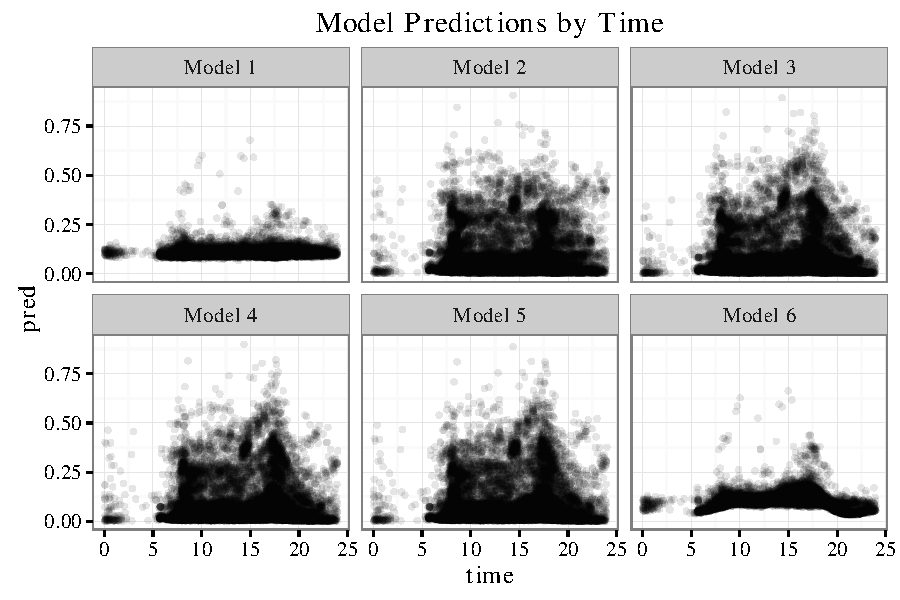
\includegraphics[angle = 0,scale = 1]{figure/time_pred_plot.pdf}
  \caption[Each of the models predictions for all rides with time of day on the x-axis.
  Notice how starting with model 2, daily trends start to emerge. This indicates that the
  rider intercepts are picking up on time of day trends, which must be reflected in riders
  typical ride.]{\normalsize{Each of the models predictions for all rides with time of day on the x-axis.
  Notice how starting with model 2, daily trends start to emerge. This indicates that the
  rider intercepts are picking up on time of day trends, which must be reflected in riders
  typical ride.}}
  \label{fig:time-pred-plot}
  \end{figure}
  
  One should be cautious about interpreting the intercepts. It's tempting
  to say they represent a riders general tendency to rate rides
  negatively, but this is ignoring their typical route. Just like how
  figure \autoref{fig:time-pred-plot} demonstrates that riders have unique
  patterns of what times of days they take rides, riders also likely have
  very particular routes that make up the majority of their rides. Because
  our models do not take into account the route, the intercepts are likely
  encoding the information about a riders typical route.
  
  The fact that riders have apparent patterns of time of ride (and very
  likely route of ride), indicates there will be some value in trying to
  differentiate the types of riders that are present in this data. Indeed,
  one way of looking at the range of probabilities of giving a negative
  rating different riders have (demonstrated in figure
  \autoref{fig:rider-pred}) is that some are more likely to offer useful
  information. In the next chapter, we will attempt to pick apart
  different groups of riders, and attempt to characterize their patterns
  of when and how long they ride.
  
  \begin{figure}[tbh]
  \centering
  \includegraphics[angle = 0,scale = 1]{figure/rider_predictions.pdf}
  \caption[Predicted probability of a negative rating for a typical ride for 
  each rider, for Model 2 and Model 4. The typical ride is a ride at noon on a 
  weekday with median length, mean temperature, and other variables at zero.]{\normalsize{Predicted probability of a negative rating for a typical ride for 
  each rider, for Model 2 and Model 4. The typical ride is a ride at noon on a 
  weekday with median length, mean temperature, and other variables at zero.}}
  \label{fig:rider-pred}
  \end{figure}
  
  \chapter{Classifying Riders}\label{classifying-riders}
  
  Given the results from last chapter, there is a clear need to understand
  what kinds of riders are in this data set. Ride Report, because they
  need to respect the privacy of their users, cannot identify individual
  riders in the data they provide to clients, yet our model results show
  that differentiating riders is crucial to getting good estimates in our
  models. However, there is one potential solution to this problem: If we
  can identify clusters of riders in the data set that give us nearly the
  same information as grouping by individuals did, these could be provided
  by Ride Report without nearly the same level of risks to user privacy as
  identifying individual riders.
  
  In this chapter, we identify predictors that differentiate types of
  riders and then use these variables to identify clusters of riders. To
  tie these predictors into our model, we test to see how these predictors
  do as rider-level predictors for the intercepts and even some
  coefficients. We also compare random intercepts with riders to random
  intercept models done by cluster.
  
  \section{Characterizing riders}\label{characterizing-riders}
  
  We characterized riders based on their rides. Ride Report does not
  collect data about their users besides their rides and email address. We
  limited our exploration to riders that had over 20 rated rides, because
  we wanted to focus on riders who had been using the app for some time
  and had an identifiable pattern of rides.
  
  Cyclists patterns in their rides are complex, particularly their time
  patterns. Computing their mean ride length for weekends was useful, but
  mean time of day for their rides does not capture anything meaningful.
  So we took care in selecting features that distinguished different rider
  patterns we saw when exploring the data and that did not have high
  covariance.
  
  \begin{figure}[htb]
  \centering
  \includegraphics{figure/time-designations.pdf}
  \caption{These intervals define the time designations we used in clustering. 
  The proportion of each riders rides in each of these time intervals made up three
  of our features.\label{fig:time-splits}}
  \end{figure}
  
  First, we define the collection of cyclist \(j\)'s rides as
  \(H_j = \{ i | j[i] = j \}\). This index set can be partitioned into the
  rides that occured on the weekend,
  \(H_j^\text{weekend} = \{ i | i \in H_j, x_i^\text{weekend} = 1\}\), and
  those that occurred on weekdays,
  \(H_j^\text{weekday} = H_j \setminus H_j^\text{weekend}\). Then we
  define the following for each rider \(j\): frequency of rides\footnote{We
    define frequency of a cyclist's rides as the number of rides divided
    by the difference between the time of the most recent ride and time of
    the first ride. (Units are arbitrary, because we standardized all of
    our rider-level variables.)} (\(u^\text{freq}_j\)), proportion of
  rides on weekdays (\(u^\text{weekend}_j\)), median length of rides on
  weekends (\(u^\text{med.len}_j\)) and weekends
  (\(u^\text{med.len.w}_j\)), variance of ride length on weekdays
  (\(u^\text{var.len}_j\)) and weekdays (\(u^\text{var.len.w}_j\)), and
  proportion of weekday rides during morning rush
  (\(u^\text{morning}_j\)), lunch rush (\(u^\text{lunch}_j\)), and evening
  rush (\(u^\text{evening}_j\)). The time intervals that describe the
  morning, lunch, and evening rush are shown in \autoref{fig:time-splits}.
  
  Selecting variables for a cluster analysis is difficult, for the reason
  that many choices about what to use are arbitrary. We have chosen these
  variables, but two important other choices remain: what scales and
  transformations should these variables have? We chose here to transform
  all variables to be approximately gaussian---eliminating the right skew
  that was present in most of these features with log and square root
  transformions---and standardizing them by subtracting their mean and
  dividing by their standard deviation. Future research may find more
  appropriate ways to select features for clustering, but in our approach
  here we stick to a naive and simple approach to see what we can learn.
  
  With the rider-level predictors in hand, we clustered the riders using
  the \(k\)-means algorithm, using Euclidean distance as the metric. To
  choose the number of clusters, we assessed the total of the sum of
  squares within each cluster for different values of \(k\), shown in
  \autoref{fig:choosing_k}, and selected \(k = 4\) as the point where we
  thought after which there was little value in more clusters.
  
  \begin{figure}[tbh]
  \centering
  \includegraphics[angle = 0,scale = 1]{figure/choice_k.pdf}
  \caption[Total within sum of squares of each cluster, by number of clusters ($k$).]{\normalsize{Total within sum of squares of each cluster, by number of clusters ($k$).}}
  \label{fig:choosing_k}
  \end{figure}
  
  \begin{figure}[htb]
  \centering
  \includegraphics[width=.33\textwidth]{figure/cluster_scatter1.pdf}\hfill
  \includegraphics[width=.33\textwidth]{figure/cluster_scatter2.pdf}\hfill
  \includegraphics[width=.33\textwidth]{figure/cluster_scatter3.pdf}
  \caption{Rider clusters identified by $k$-means clustering. The triangles represent
  the centroids (computed as the mean) of the cluster members. \label{fig:cluster-scatter}}
  \end{figure}
  
  Looking at \autoref{fig:cluster-scatter}, the clusters split the data
  into the four quadrants of the first two principal components of the
  rider data. This makes sense, given our scree plot only showed very
  differences in total within sum of squares at \(k\) got larger. Despite
  having failed to identify distinct cluters, studying these different
  groups, can still off some valuable insight into how cylists differ in
  their ride patterns.
  
  \autoref{fig:cluster-patterns} shows the complex patterns the different
  groups display. Clusters 1 and 3 seem to be the groups that are the most
  consistent cummuters, but are differtiated the the typical length of
  their weekend. Clusters 2 and 4 show much more variance in the timing of
  their weekdays rides, with cluster 2 having more consistent long lengths
  for their weekend rides.
  
  \begin{figure}[bht]
  \centering
  \includegraphics[angle = 0,scale = 1]{figure/cluster_patterns.pdf}
  \caption[Patterns of ride length and ride time of day for each cluster..]{\normalsize{Patterns of ride length and ride time of day for each cluster..}}
  \label{fig:cluster-patterns}
  \end{figure}
  
  \section{Models with Rider-level
  predictors}\label{models-with-rider-level-predictors}
  
  We now have several variables that differentiate riders. How well do
  they predict our rider intercepts?
  
  Now let \(U_j\) be the vector of rider-level variables. Then our model
  will be
  
  \begin{equation}
  Y_i \sim \text{Bernoulli} \left( \text{logit}^{-1}
  (\alpha_{j[i]} + X_i \beta) \right),
  \end{equation}
  
  where,
  
  \begin{equation}
  \alpha_j \sim N(\gamma_0 + U_j \gamma)
  \end{equation}
  
  This model should be comparable to Model 2.\footnote{Though we would
    prefer to use a model similar to Model 4 from the previous chapter
    (the one with smoothing splines for time of day) the current additive
    mixed models package \texttt{gamm4} (which uses \texttt{lme4} to fit
    the mixed models part) does not support estimating the variability in
    group-level estimates. Instead, we fit these models in Stan, a
    probabilitic modeling language that does full Bayesian statistical
    inference with Markov-chain Monte Carlo sampling. Unfortunately, in
    this package, smoothing splines would have to be coded by hand and we
    lacked the expertise to write the functions to fit smoothing splines
    ourselves.}
  
  \begin{table}[htb]
  \caption{Estimates of rider level predictors. \label{tab:rider-level-estimates}}
  \centering
  \begin{tabular}{lrrrr}
  \toprule
  \textbf{Parameter} & Estimate & 2.5\% percentile & 97.5\% percentile\\
  \midrule
  $\gamma^\text{freq}$ & 0.08 & -0.19 & 0.35\\
  $\gamma^\text{weekend}$ & -0.13 & -0.50 & 0.35\\
  $\gamma^\text{morning}$ & 0.06 & -0.22 & 0.34\\
  $\gamma^\text{afternoon}$ & 0.13 & -0.20 & 0.44\\
  $\gamma^\text{evening}$ & -0.02 & -0.31 & 0.27\\
  $\gamma^\text{med.len}$ & 0.01 & -0.25 & 0.29\\
  $\gamma^\text{med.len.w}$ & 0.08 & -0.19 & 0.36\\
  $\gamma^\text{var.len}$ & 0.07 & -0.15 & 0.31\\
  $\gamma^\text{var.len.w}$ & -0.15 & -0.47 & 0.17\\
  $\gamma_0$ & -2.99 & -3.29 & -2.69\\
  $\sigma_\alpha$ & 1.47 & 1.27 & 1.69\\
  \bottomrule
  \end{tabular}
  \end{table}
  
  The ride-level predictor coefficients from the fitted model, are
  unimpressive. The variance in the rider intecepts not captured by the
  predictors, quantified with \(\sigma_\alpha\), is high.
  
  \section{Cluster Intercepts Versus Rider
  Intercepts}\label{cluster-intercepts-versus-rider-intercepts}
  
  Do these clusters provide similarly useful information that we got from
  introducing rider intercepts? Naturally, we expect that a model with
  cluster intercepts will do worse than rider intercepts simply by virtue
  of less flexibility. Having only four different intercepts rather than
  hundreds doesn't sound like a recipe for success. But perhaps there is
  still a significant benefit.
  
  There isn't. We computed Model 7, which is identical to Model 4 from the
  previous chapter, but has random intercepts by cluster rather than
  rider. Model 7 performed slightly better than Model 6---which only had a
  fixed intercept---but nowhere near as well as Model 4. The separation
  plots, \(\log (\mathcal{L})\), AIC, and AUC measures, shown in
  \autoref{tab:cluster-model-fits}, all demonstrate this clearly.
  
  \chapter{Modeling Missing Response}\label{modeling-missing-response}
  
  We have a significant portion of observations with no response. But we
  do have all the predictors for every observation. So just as we built a
  model to predict the rating, can we build a model to predict whether a
  rider will give a rating? Going further, could we combine our rating
  model and nonresponse model into one model, such that our predictions
  for ratings will take into account biases in nonresponse?
  
  We attempt to address these two questions in this chapter. The methods
  we present in this chapter could improve inference greatly on this data,
  but we do have concerns about the current quality of the data for which
  there are no reponses. As mentioned in Chapter 1, one big problem with
  data collection is that rides are often misclassified as bike rides when
  they are actually car rides or rides on public transit. We suspect that
  many of the unrated rides are rides that were misclassified as bike
  rides, and thus were not rated by the rider. (We assume that riders
  don't often go through the effort of correcting the classification of
  rides and know not to rate rides that weren't bike rides.) That being
  said, this issue could potentially be fixed and these methods used again
  in the future.
  
  \section{What could possibly go
  wrong?}\label{what-could-possibly-go-wrong}
  
  We focus on the situation we have, where our response variable \(y_i\)
  has missing values. Define the vector \(R = (r_1, r_2, \ldots, r_n)\)
  such that
  
  \begin{equation}
  r_i = \left\{ \begin{array}{ll}
  1, & \text{if } y_i \text{ is missing};\\
  0, & \text{if } y_i \text{ is observed};
  \end{array}
  \right.
  \end{equation}
  
  Rubin classifies missing data into three situations\footnote{Little and
    Rubin (1987) (page 14)}:
  
  \begin{enumerate}
  \def\labelenumi{\arabic{enumi}.}
  \tightlist
  \item
    \textbf{Missing Completely at Random (MCAR)}, where \(R\) is
    independent of \(Y\) and the predictors \(X\). \emph{i.e.},
    \(\mathbb{P} (R = 1| Y, X) = \mathbb{P}(R = 1\).)
  \item
    \textbf{Missing at Random (MAR)}, where \(R\) is independent of \(Y\),
    but may depend on \(X\), \emph{i.e.}
    \(\mathbb{P} (R = 1 |Y, X) = \mathbb{P} (R = 1 | Y, )\)
  \item
    \textbf{Nonignorable, or not MCAR nor MAR}, where \(R\) is dependent
    on \(Y\).
  \end{enumerate}
  
  We believe that rider ratings may be correlated with nonresponse. One
  explination: riders who have a unpleasant experience on the road, might
  feel more incentive to report their experience on the app than those who
  had a ride that was uneventful. This motivates our exploration of
  missing data models, though, of course, is by no means evidence of
  nonignorable missing data.
  
  If missing data is nonignorable, what could go wrong with our models?
  Let look at a toy example. Define the data set of \(n\) observations
  with \(X \in \mathbb{R}^n\), \(Y \in \{0,1\}^n\), and \(R\) defined as
  before, where \[x_i \sim \text{Normal}(0,1),\]
  \[y_i \sim \text{Binomial}(\text{logit}^{-1} (4x_i)),\]
  \[r_i \sim \text{Binomial}(0.3 + 0.4 y_i),\] for \(i = 1, \ldots, n\).
  
  \begin{figure}[htb]
  \centering
  \includegraphics{figure/missing_model1_estimates.pdf}
  \caption[Simulated example of biased estimates from nonignorable missing data.]{Simulated example of logistic regression fits to a model with nonignorable
  missing response. One data set of size $n = 10^4$ was computed from the toy data model.
  We then recomputed $R$ 1,000 times, each time fitting a simple logistic regression
  model to $Y$ and $X$.}
  \end{figure}
  
  If we attempt to fit a logistic regression model to this data, our
  slopes will be unbiased but our estimate of the intercept will be very
  biased. \autoref{fig:missing-model1-estimates} shows the results of a
  simulation, computing the slope and intercepts for 1,000 different
  patterns of missing data for the same generated data set generated from
  our toy data model.
  
  It makes sense that we are underestimating our intercept. The intercept
  can be interpretted as the base rate, and if value of \(y_i = 1\) are
  more likely to be missing, the overall rate we observe will be lower.
  
  Clearly, if we have nonignorable missing response, we are in a bad
  situation. Having missingness depend on \(Y\) leads to biased estimates
  of our intercepts when we fit models. But we do have all of our
  predictors of \(y\), with no missingness. Could we leverage our
  understanding of how \(X\) predicts \(Y\) to understand the patterns of
  missing response?
  
  \section{Using Expectation Maximization}\label{em-algorithm}
  
  We can try to perform the expectation maximization algorithm here, using
  the weighting method proposed by Ibrahim and Lipsitz\footnote{Ibrahim
    and Lipsitz (1996)}. Let \(y_i\) be our binary response and \(x_i\) be
  our predictors. With these we have our complete data logistic regression
  model \(f(y_i \;|\; x_i, \beta)\), where \(\beta\) is a vector of
  parameters in the complete data model.
  
  We then specify a logistic regression model for missingness (the
  \(r_i\)'s): \(f(r_i \;|\; x_i, y_i, \alpha)\), where \(\alpha\) is the
  vector of parameters in the missingness model.
  
  We begin the algorithm by getting our first estimates of \(\alpha\) and
  \(\beta\). We obtain \(\beta^{(1)}\) by estimating \(\beta\) with only
  the non-missing data. We can then estimate the \(y_i\) for the missing
  data using \(\beta^{(1)}\), and then use those estimates to compute
  \(\alpha^{(1)}\).
  
  For the E-step, we compute weights for each observation with missing
  response
  
  \begin{equation}
  w_{i\: y_i}^{(t)} = 
  f(y_i \;|\; r_i, x_i, \alpha^{(t)}, \beta^{(t)}) =
  \frac{f(y_i \;|\; x_i, \beta^{(t)}) f(r_i \;|\; x_i, y_i, \alpha^{(t)})}{
  \sum_{y_i = 0}^1
  f(y_i \;|\; x_i, \beta^{(t)}) f(r_i \;|\; x_i, y_i, \alpha^{(t)})
  }.
  \end{equation}
  
  (For observed responses, \(w_{i\: y_i}^{(t)} = 1\).) We can compute
  \(f(y_i \;|\; x_i, \beta^{(t)})\) and
  \(f(r_i \;|\; x_i, y_i, \alpha^{(t)})\) by making use of predictions
  from regression models. So in \textit{R}, we can fit models and use the
  \texttt{predict()} function to get our probabilities from each of these
  models.
  
  For the M-step, we find our next estimates of the parameters,
  \(\alpha^{(t + 1)}\) and \(\beta^{(t + 1)}\), by maximizing
  
  \begin{equation}
  Q(\alpha, \beta \;|\; \alpha^{(t)}, \beta^{(t)}) =
  \sum_{i = 1}^n \sum_{y_i \in \{0,1\}} w_{iy_i}^{(t)} 
  l(\alpha, \beta | x_i, y_i, r_i).
  \end{equation}
  
  We do this by first by estimating \(\beta^{(t + 1)}\) using weighted
  maximum likelihood for the complete data model, and then estimating
  \(\alpha^{(t + 1)}\) using the same method. To maximize
  \(l(\alpha, \beta | x_i, y_i, r_i)\), we maximize the product of their
  likelihoods,
  \[l(\alpha, \beta | x_i, y_i, r_i) = l(\beta | x_i, y_i) l(\alpha | r_i, x_i, y_i),\]
  which we can maximize by maximize each of the likelihoods separately
  because our estimates of \(\alpha\) and \(\beta\) are independent. This
  allows us to use any package that can fit models by maximum likelihood
  estimation using weights for the observations, which includes all of the
  model fitting packages we used in Chapter 3.
  
  In order to create the data to fit these models, we create an augmented
  data set where each observation missing the response is recorded as two
  rows, which represent the two possible values of the response, and also
  contain the weights computed in the E-step.
  
  \begin{figure}[htb]
  \centering
  \caption{Creation of augmented data set for the weighted method of the EM algorithm for missing response data. \label{fig:augmented-data}}
  \begin{tabular}{lcl}
  \toprule
  \textbf{Original Data} &  & \textbf{Augmented Data}\\
  \midrule
  
  \begin{tabular}{lll}
  $y_i$ & $x_i$ & $r_i$\\
  \midrule
  1 & 2.4 & 0\\
  0 & 1.3 & 0\\
  NA & -0.4 & 0\\
  & &
  \end{tabular}
  &
  $\to$
  &
  \begin{tabular}{llll}
  $y_i$ & $x_i$ & $r_i$ & $w_i$\\
  \midrule
  1 & 2.4 & 0 & 1\\
  0 & 1.3 & 0 & 1\\
  1 & -0.4 & 0 & 0.2\\
  0 & -0.4 & 0 & 0.8
  \end{tabular}\\
  \bottomrule
  \end{tabular}
  \end{figure}
  
  We repeat the E and M step until the values of \(\alpha\) and \(\beta\)
  converge.
  
  As an example, we simulated a dataset from the same model we presented
  earlier of size \(10^4\). Of those observations, 6,252 were missing. As
  shown in \autoref{tab:EM-sim}, the estimate for the intercept in the
  model that only considers the complete data is way off, but the model
  resulting from the EM algorithm are nearly as accurate as the model
  computed fit to the full data (with missing values filled in from the
  original data model.) The missing data model is also able to get
  accurate estimates of the parameters that define the missing data
  mechanism, but the estimates are quite uncertain.
  
  \begin{table}[htb]
  \caption{Coefficients for models fit to simulated data set ($\pm$ twice the
  standard error.) \label{tab:EM-sim}}
  \centering
  \begin{tabular}{lrrrr}
  \toprule
  Model & $\hat{\beta}_0$ & $2 \cdot SE_{\hat{\beta}_0}$  & 
  $\hat{\beta}_X$ &  $2 \cdot SE_{\hat{\beta}_X}$\\
  \midrule
  Actual & 0 & -- & 4 & --\\
  Full Data Model & $-0.009$ &  $0.065$ & $3.881$ &  $0.080$\\
  Complete Data Model & $-0.278$ & $0.106$ & $3.819$ &  $0.259$\\
  EM Final Model & $0.042$ & $0.065$ & $3.814$ &  $0.157$\\
  \bottomrule
  \end{tabular}
  \end{table}
  
  \begin{table}[htb]
  \caption{Estimates for missing data mechanism. \label{tab:EM-sim-missing}}
  \centering
  \begin{tabular}{lrrrr}
  \toprule
  Model & $\hat{\alpha}_0$ & $2 \cdot SE_{\hat{\alpha}_0}$ 
  & $\hat{\alpha}_Y$ &  $2 \cdot SE_{\hat{\alpha}_Y}$\\
  \midrule
  Actual & 0.3 & -- & 0.4 & --\\
  EM Missing Data Model & $0.263$ & $0.132$ & $0.530$ &  $0.268$\\
  \bottomrule
  \end{tabular}
  \end{table}
  
  \section{Creating a Missing Data
  Model}\label{creating-a-missing-data-model}
  
  In order to perform the algorithm, we need to specify a model for
  nonresponse. We will the same predictors that we do in Model 4 for ride
  rating---including a smoothing spline for time of day for weekdays and
  weekends---except we do not use random rider intercepts. We can specify
  a basic nonresponse model as
  
  \begin{equation}
  r_i \sim Bernoulli(\text{logit}^{-1} (\alpha + x_i \beta + \mathcal{S}(t_i))).
  \end{equation}
  
  For the EM algorithm, we use Model 4 as our ride rating model and use
  the following model for the rating nonresponse mechanism:
  
  \begin{equation}
  r_i \sim Bernoulli(\text{logit}^{-1} (\alpha + y_i \beta_Y + x_i \beta + \mathcal{S}(t_i))).
  \end{equation}
  
  \begin{table}[htb]
  \caption{Estimates for ride rating nonresponse mechanism. \label{tab:nonresponse-estimates}}
  \centering
  \begin{tabular}{lrrrr}
  \toprule
  \textbf{Parameter} & \textbf{Basic Nonresponse Model} & \textbf{EM Nonresponse Model}\\
  \midrule
  Log(Length) & -0.377 & -0.365\\
  Mean Temperature & 0.071 & -0.068\\
  Mean Wind Speed & 0.004 & ???\\
  Max Gust Speed & 0.004 & 0.008\\
  Rainfall & -0.002 & -0.003\\
  Rainfall 4-Hour & 0.008 & 0.008\\
  Intercept & 0.072 & -0.060\\
  \bottomrule
  \end{tabular}
  \end{table}
  
  \begin{table}[htb]
  \caption{Ride rating model estimates after EM algorithm \label{tab:em-model-estimates}}
  \centering
  \begin{tabular}{lrrrr}
  \toprule
  \textbf{Parameter} & \textbf{Model 4} & \textbf{EM Model}\\
  \midrule
  Log(Length) & -0.196 & \\
  Mean Temperature & 0.100 & \\
  Mean Wind Speed & -0.001 & \\
  Max Gust Speed & 0.006 & \\
  Rainfall & -0.002 & \\
  Rainfall 4-Hour & 0.025 & \\
  Intercept & -2.987 & \\
  \bottomrule
  \end{tabular}
  \end{table}
  
  \chapter{Unfinished Work: Incorporating
  Routes}\label{unfinished-work-incorporating-routes}
  
  These models so far do not incorporate route. Unfortunately, I was not
  able to get to models that actually do. The data transformations
  necessary were more than I could reasonably do in addition to the other
  parts of developing the models. So I leave the models as they are, but
  here I explain some of my work toward the goal of incorporating routes
  and describe some potential modeling approaches.
  
  \section{Regression Terms for Road
  Segments}\label{regression-terms-for-road-segments}
  
  Now we have the task of incorporating our knowledge of riders' routes
  into our regression. Our approach here will be to consider routes as
  sequences of discrete road segments, each of which have known
  properties. This is convenient because we have such data about roads
  that give us bike lanes, road size, etc. It is even possible for us to
  calculate popularity of particular segments easily.
  
  Assume we have \(K\) total road segments in our road network and for
  each ride we have \(\Omega_i \subseteq \{1, \ldots, K\}\), the set of
  road segments that are in the route of ride \(i\). Let \(l_k\) be the
  length of the \(k\)th segment and define the length of ride \(i\) to be:
  
  \[ L_i = \sum_{k \in \Omega_i} l_k.\]
  
  For the \(k\)th road segment, define the m-dimensional vector
  \(W_k = W_k^1, W_k^2, \ldots, W_k^m\) road segment-level predictors.
  Then we shall define the term in our regression for the route of ride
  \(i\) as
  
  \[ R_i = \frac{1}{L_i} \sum_{k \in \Omega_i} l_k W_k \beta^{\text{road}},\]
  
  Where \(\beta^{\text{road}}\) is a vector of coefficients for the road
  segment level predictors. When actually computing this value, it may be
  convenient to factor out the \(\beta^{\text{road}}\)
  
  \backmatter
  
  \chapter{References}\label{references}
  
  \noindent
  
  \setlength{\parindent}{-0.20in} \setlength{\leftskip}{0.20in}
  \setlength{\parskip}{8pt}
  
  \hypertarget{refs}{}
  \hypertarget{ref-cressie2011}{}
  Cressie, Noel, and Cristopher K. Wikle. 2011. \emph{Statistics for
  Spatio-Temporal Data}. John Wiley \& Sons.
  
  \hypertarget{ref-esarey2012}{}
  Esarey, Justin, and Andrew Pierce. 2012. ``Assessing Fit Quality and
  Testing for Misspecification in Binary-Dependent Variable Models.''
  \emph{Political Analysis} 20 (4): 480--500.
  
  \hypertarget{ref-gelman}{}
  Gelman, Andrew, and Jennifer Hill. 2006. \emph{Data Analysis Using
  Regression and Multilevel/Hierarchical Models}. The Edinburgh Building,
  Cambridge CB2 8RU, UK: Cambridge University Press, New York.
  
  \hypertarget{ref-greenhill2011}{}
  Greenhill, Brian, Michael D. Ward, and Audrey Sacks. 2011. ``The
  Separation Plot: A New Visual Method for Evaluating the Fit of Binary
  Models.'' \emph{American Journal of Political Science} 55 (4). Midwest
  Political Science Association: 991--1002.
  
  \hypertarget{ref-ibrahim1996}{}
  Ibrahim, Joseph G., and Stuart R. Lipsitz. 1996. ``Parameter Estimation
  from Incomplete Data in Binomial Regression When the Missing Mechanism
  Is Nonignorable.'' \emph{Biometrics} 52 (3): 1071--8.
  
  \hypertarget{ref-little1987}{}
  Little, Roderick J.A., and Donald B. Rubin. 1987. \emph{Statistical
  Analysis with Missing Data}. John Wiley \& Sons.
  
  \hypertarget{ref-mackaronis2013}{}
  Mackaronis, Julia E., Donald S. Strassberg, Jeanne M. Cundiff, and
  Deanna J. Cann. 2013. ``Beholder and Beheld: A Multilevel Model of
  Perceived Sexual Appeal.'' \emph{Archives of Sexual Behavior}, October.
  
  \hypertarget{ref-cosmaadditive}{}
  Shalizi, Cosma. 2013a. ``Additive Models.''
  \url{http://www.stat.cmu.edu/~cshalizi/uADA/13/lectures/ch09.pdf}.
  
  \hypertarget{ref-cosmasplines}{}
  ---------. 2013b. ``Splines.''
  \url{http://www.stat.cmu.edu/~cshalizi/uADA/13/lectures/ch08.pdf}.
  
  \hypertarget{ref-wood2006}{}
  Wood, Simon. 2006. \emph{Generalized Additive Models: An Introduction
  with R}. CRC press.


  % Index?

\end{document}

